\subsubsection{{Segmentação de imagens}}

De forma a dar continuidade ao ciclo de processamento de imagem e verificação desta, usa-se métodos de \textit{pixels} e tonalidades seguindo os padrões propostos. A análise deve prosseguir de forma minuciosa para então, processar seus detalhes.

A segmentação veio para aprimorar a parte de processamento, auxiliando na detecção de maiores detalhes e reduzindo tempo de processamento. Isso ocorre porque a segmentação é a área que tem por responsabilidade dividir a imagem em várias partes significativas, separando as de interesse dentro desta \cite{FILHO1999}.

No entanto, a segmentação exige um processamento muito grande para analisar a imagem sugerida. Sendo assim, o nível no qual será feito essa subdivisão de imagem depende muito da ocasião e do problema que está sendo proposto para resolver. De acordo com \citeonline{GONZALEZ2002}, para não ocorrer perca desnecessária de processamento e, consequentemente, perda de tempo, a segmentação deve parar assim que os objetos de interesse da aplicação forem isolados.

Portanto, dentro da segmentação existem métodos que podem ser seguidos a fim de analisar detalhadamente cada figura. Segundo \citeonline{MORGAN2008}, as classificações dos métodos utilizados na segmentação são definidos como interativos ou automáticos. Basicamente, a diferença entre os dois são bem simples: um é executado através de intervenções humanas e o outro não.

Além disso, no processo de segmentação interativa, o usuário utiliza ferramentas e técnicas que se adéquam da melhor forma a sua imagem e necessidade, solucionando-a da melhor forma possível. Esse método normalmente é mais utilizado para solucionar problemas específicos, onde as condições da imagem podem interferir drasticamente na análise final da mesma como, por exemplo, \textit{softwares} que analisam imagens de doenças graves adquiridas através de ressonâncias, onde a aplicação pode confundir um ruído ou uma área com má iluminação em um ponto de análise clínica.

Já o processo de segmentação automática onde, na maioria das vezes, utilizam robôs para realizar as tomadas de decisões através dos resultados obtidos na análise da imagem, inexiste interferência humana no processo. Esse método está sendo aplicado, por exemplo, em carros autônomos, onde o mesmo identifica a presença de obstáculos em sua frente e com base no obstáculo e na proporção do mesmo, uma ação e tomada.

Para complementar, \citeonline{MORGAN2008} enfatiza que existem métodos que são classificados de acordo com a representação dos objetos a serem segmentados, que são os métodos de borda ou orientados a regiões.

O processo de segmentação baseado no método de bordas utiliza basicamente pontos de uma imagem onde ocorre alguma intensidade de luz, ou seja, onde os \textit{pixels} estão mais visíveis, realçando a borda do objeto e consequentemente diferenciando do fundo da imagem. Pode-se também localizar uma borda através de uma mudança brusca nos tons de cinza, gerados por regiões distintas. Com base na borda que foi extraída da imagem, tem-se então uma imagem topográfica do objeto que será analisado.

A Figura 8 mostra como funciona uma análise baseada no método de bordas.

\clearpage

\begin{figure}[!htb]
\caption{{\footnotesize Resultado de uma análise feita utilizando o método de bordas.}}
 
\centering % para centralizarmos a figura
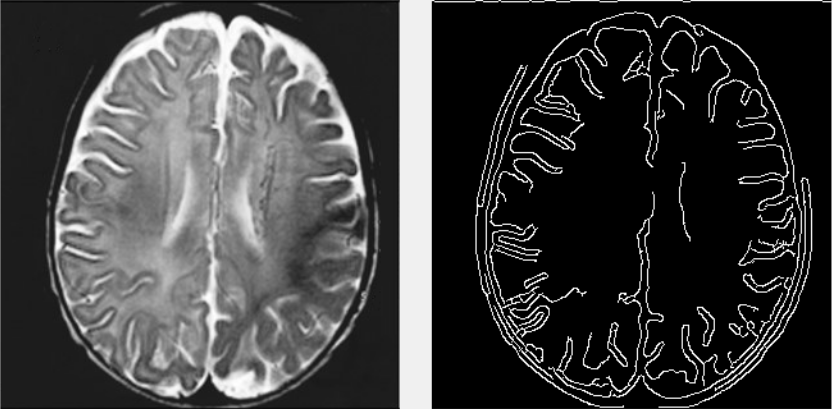
\includegraphics[width=12cm]{revisao-bibliografica/Figuras/MetodoDeBorda.png}% leia abaixo
\label{figura:figura6}

\centering \subfloat {\footnotesize { Fonte: \cite{FREITAS2016} }}
{
\label{figura:figura6}
}
\end{figure}

Conforme \citeonline{MORGAN2008} enfatiza em seu artigo, o método orientado a regiões é dividido em três abordagens relevantes: classificação por \textit{pixel}, agregação de \textit{pixel} e \textit{split-and-merge} (Divisão e conquista).

A descrever cada uma das abordagens de forma didática, a classificação por \textit{pixel} nada mais é que a identificação de características presentes na imagem como, por exemplo, cor, texturas, a fim de classificar os \textit{pixels} de acordo com as várias possibilidades de classes ou objetos da imagem.

Na abordagem de agregação por \textit{pixel} o objetivo é encontrar um \textit{pixel} dentro da imagem e, a partir desse \textit{pixel}, ocorre o crescimento de regiões conexas. O desenvolvimento das regiões acontece ate alcançar o critério de parada do crescimento, onde estará representado um objeto dentro da imagem.

Já a segmentação utilizando a bordagem \textit{split-and-merge} é mais complexa. Segundo \citeonline{VENTURA2009}, ao aplicar essa abordagem de segmentação, o objetivo final consiste em conseguir subdividir a imagem em vários quadrantes que satisfaça uma prioridade. Apos a concretização desta tarefa, realiza-se a verificação de cada quadrante, observando se este atende ou não a prioridade definida. Caso o quadrante não satisfaça a prioridade, a subdivisão acontece novamente em busca de outros quadrantes.

Por fim, o processo de fusão é realizado, acontecendo então o agrupamento das partes similares, ou seja, que atende as prioridades definidas. Esse processo só finaliza quando não existe nenhuma possibilidade de realizar divisões ou agrupamentos.